
%----------------------------------------------------------------------------------------
%	PACKAGES AND OTHER DOCUMENT CONFIGURATIONS
%----------------------------------------------------------------------------------------

\documentclass[12pt]{article} % Default font size is 12pt, it can be changed here
\usepackage{hyperref}
\usepackage{amsmath}
\usepackage[margin=1.4in]{geometry} % Required to change the page size to A4
\geometry{a4paper} % Set the page size to be A4 as opposed to the default US Letter
\usepackage{longtable}
\usepackage{graphicx} % Required for including pictures
\usepackage{enumerate}
\usepackage{float} % Allows putting an [H] in \begin{figure} to specify the exact location of the figure
\usepackage{wrapfig} % Allows in-line images such as the example fish picture
\usepackage{lipsum} % Used for inserting dummy 'Lorem ipsum' text into the template

\linespread{1.5} % Line spacing

%\setlength\parindent{0pt} % Uncomment to remove all indentation from paragraphs

\graphicspath{{./Pictures/}} % Specifies the directory where pictures are stored
\begin{document}

%----------------------------------------------------------------------------------------
%	TITLE PAGE
%----------------------------------------------------------------------------------------

\begin{titlepage}

\newcommand{\HRule}{\rule{\linewidth}{0.5mm}} % Defines a new command for the horizontal lines,
%change thickness here
\center % Center everything on the page

\includegraphics[width=\textwidth]{Glasgow}\\[1.5cm]
\textsc{\LARGE IT Architecture 4/M}\\[0.5cm] % Major heading such as course name
\textsc{\Large Individual Report}\\[0.5cm] % Minor heading such as course title

\HRule \\[0.4cm]
{ \huge \bfseries Discussion on the IBM workshops}\\[0.4cm] % Title of your document
\HRule \\[1.5cm]

\begin{minipage}{0.4\textwidth}
\begin{flushleft} \large
\emph{Author:}\\
Garry \textsc{Sharp}\\
0801585s\\ % Your name
\end{flushleft}
\end{minipage}
~
\begin{minipage}{0.4\textwidth}
\begin{flushright} \large
\emph{Supervisors:} \\
Dr. K. \textsc{Renaud}\\ % Supervisor's Name
Dr. P. \textsc{Tso}\\ % Supervisor's Name
\end{flushright}
\end{minipage}\\[4cm]

{\large \today}\\[3cm] % Date, change the \today to a set date if you want to be precise

\vfill % Fill the rest of the page with whitespace

\end{titlepage}

%----------------------------------------------------------------------------------------
%	TABLE OF CONTENTS
%----------------------------------------------------------------------------------------

\newpage
\tableofcontents % Include a table of contents

\newpage
\section{Overview}

During the course of this report I will be analysing various aspects of the two IBM architecture days, but should start by saying that on the whole, the experience was informative, interesting, stimulating and fun. I will focus and analyse three main parts of the exerpience, the IBM mini-lectures \& content, the activities \& team work, and finally the deliverable presentations.

\section{IBM mini-lectures and content}
This, of course, was the backbone to the entire two days, with IBM representitives aiding students throughout the day. Before each of the tasks we were given to do, we were given a mini-lecture which was essentially a summary of various concepts that had been taught earlier in the semester. These were extremely useful and if we had not been presented with such material before going into each of the tasks, I believe that the quality of work produced by the various teams would not be to the standard displayed during the workshops. All in all the content that was covered over the 2 days was presented in a logical ordering making the progression moving from task to task seem very natural. This leads me onto my next thought which is that of how the scheduling and timetabling of the workshops. 

Most of the tasks we had to do involved creating some kind of diagramatic representation of an aspect of the system and then presenting it to the IBM team and other groups, receiving very useful and valid feedback afterwards. As I mentioned before, the ordering of the tasks was very well organised, this was of particular significance in our first team exercise where we had to come up with a list of questions regarding the system proposition in order to better glean a list of requirements from the information that was available to us.

This was an excellent first task to be given as it was reasonably straightforward, providing time for team members to familiarise themselves with other members. The tasks from there on out either developed in complexity or were more time-focussed, essentailly culminating in a 15 minute presentation that had to be prepared in two hours. I will discuss the presentation aspect of the IBM workshops later in the report.

Perhaps my personal favourite of the day as whole though, is that we were given a rare opportunity to design a pseudo-system that emulates that of a real life system. It seemed to me that there was a concerted effort to ensure that the days incorporated a strong element of realism in each of the tasks (a good example of this would be each of the IBM staff adopting the role of the police force when we had a Q\&A session in task 1 to get a more comprehensive understanding of the key requirements).

\section{Activities and Team Work}

As I have already mentioned, all activities during the two days were centred around completing mini-activities in a group, before delivering a final presentation based on what we have produced from these activities. It would, therefore, be very reasonable to assume that good team skills would be highly advantageous. Although I would ideally like to attribute the good team dynamic to my own soft skill set, I think that realistically I was very lucky with the other members of the team that I had the pleasure to work with. Indeed, apart from one very minor argument regarding how I thought we should approach the final presentation, everyone seemed very agreeable to other members' ideas and intercommunication within the team was very relaxed and informal whilst still maintaining an underlying effectiveness.

\subsection{Role within the team}

The role that I had within the team was not fixed, that is to say, the structure that we employed was very relaxed and who presented which diagrams was done on an ad hoc basis. Usually, there was a member of the team that felt particularlly comfortable describing a certain diagram or exercise and they presumed the role of unofficial team leader for the duration of that exercise. 

\begin{wrapfigure}{r}{0.5\textwidth}
\begin{center}
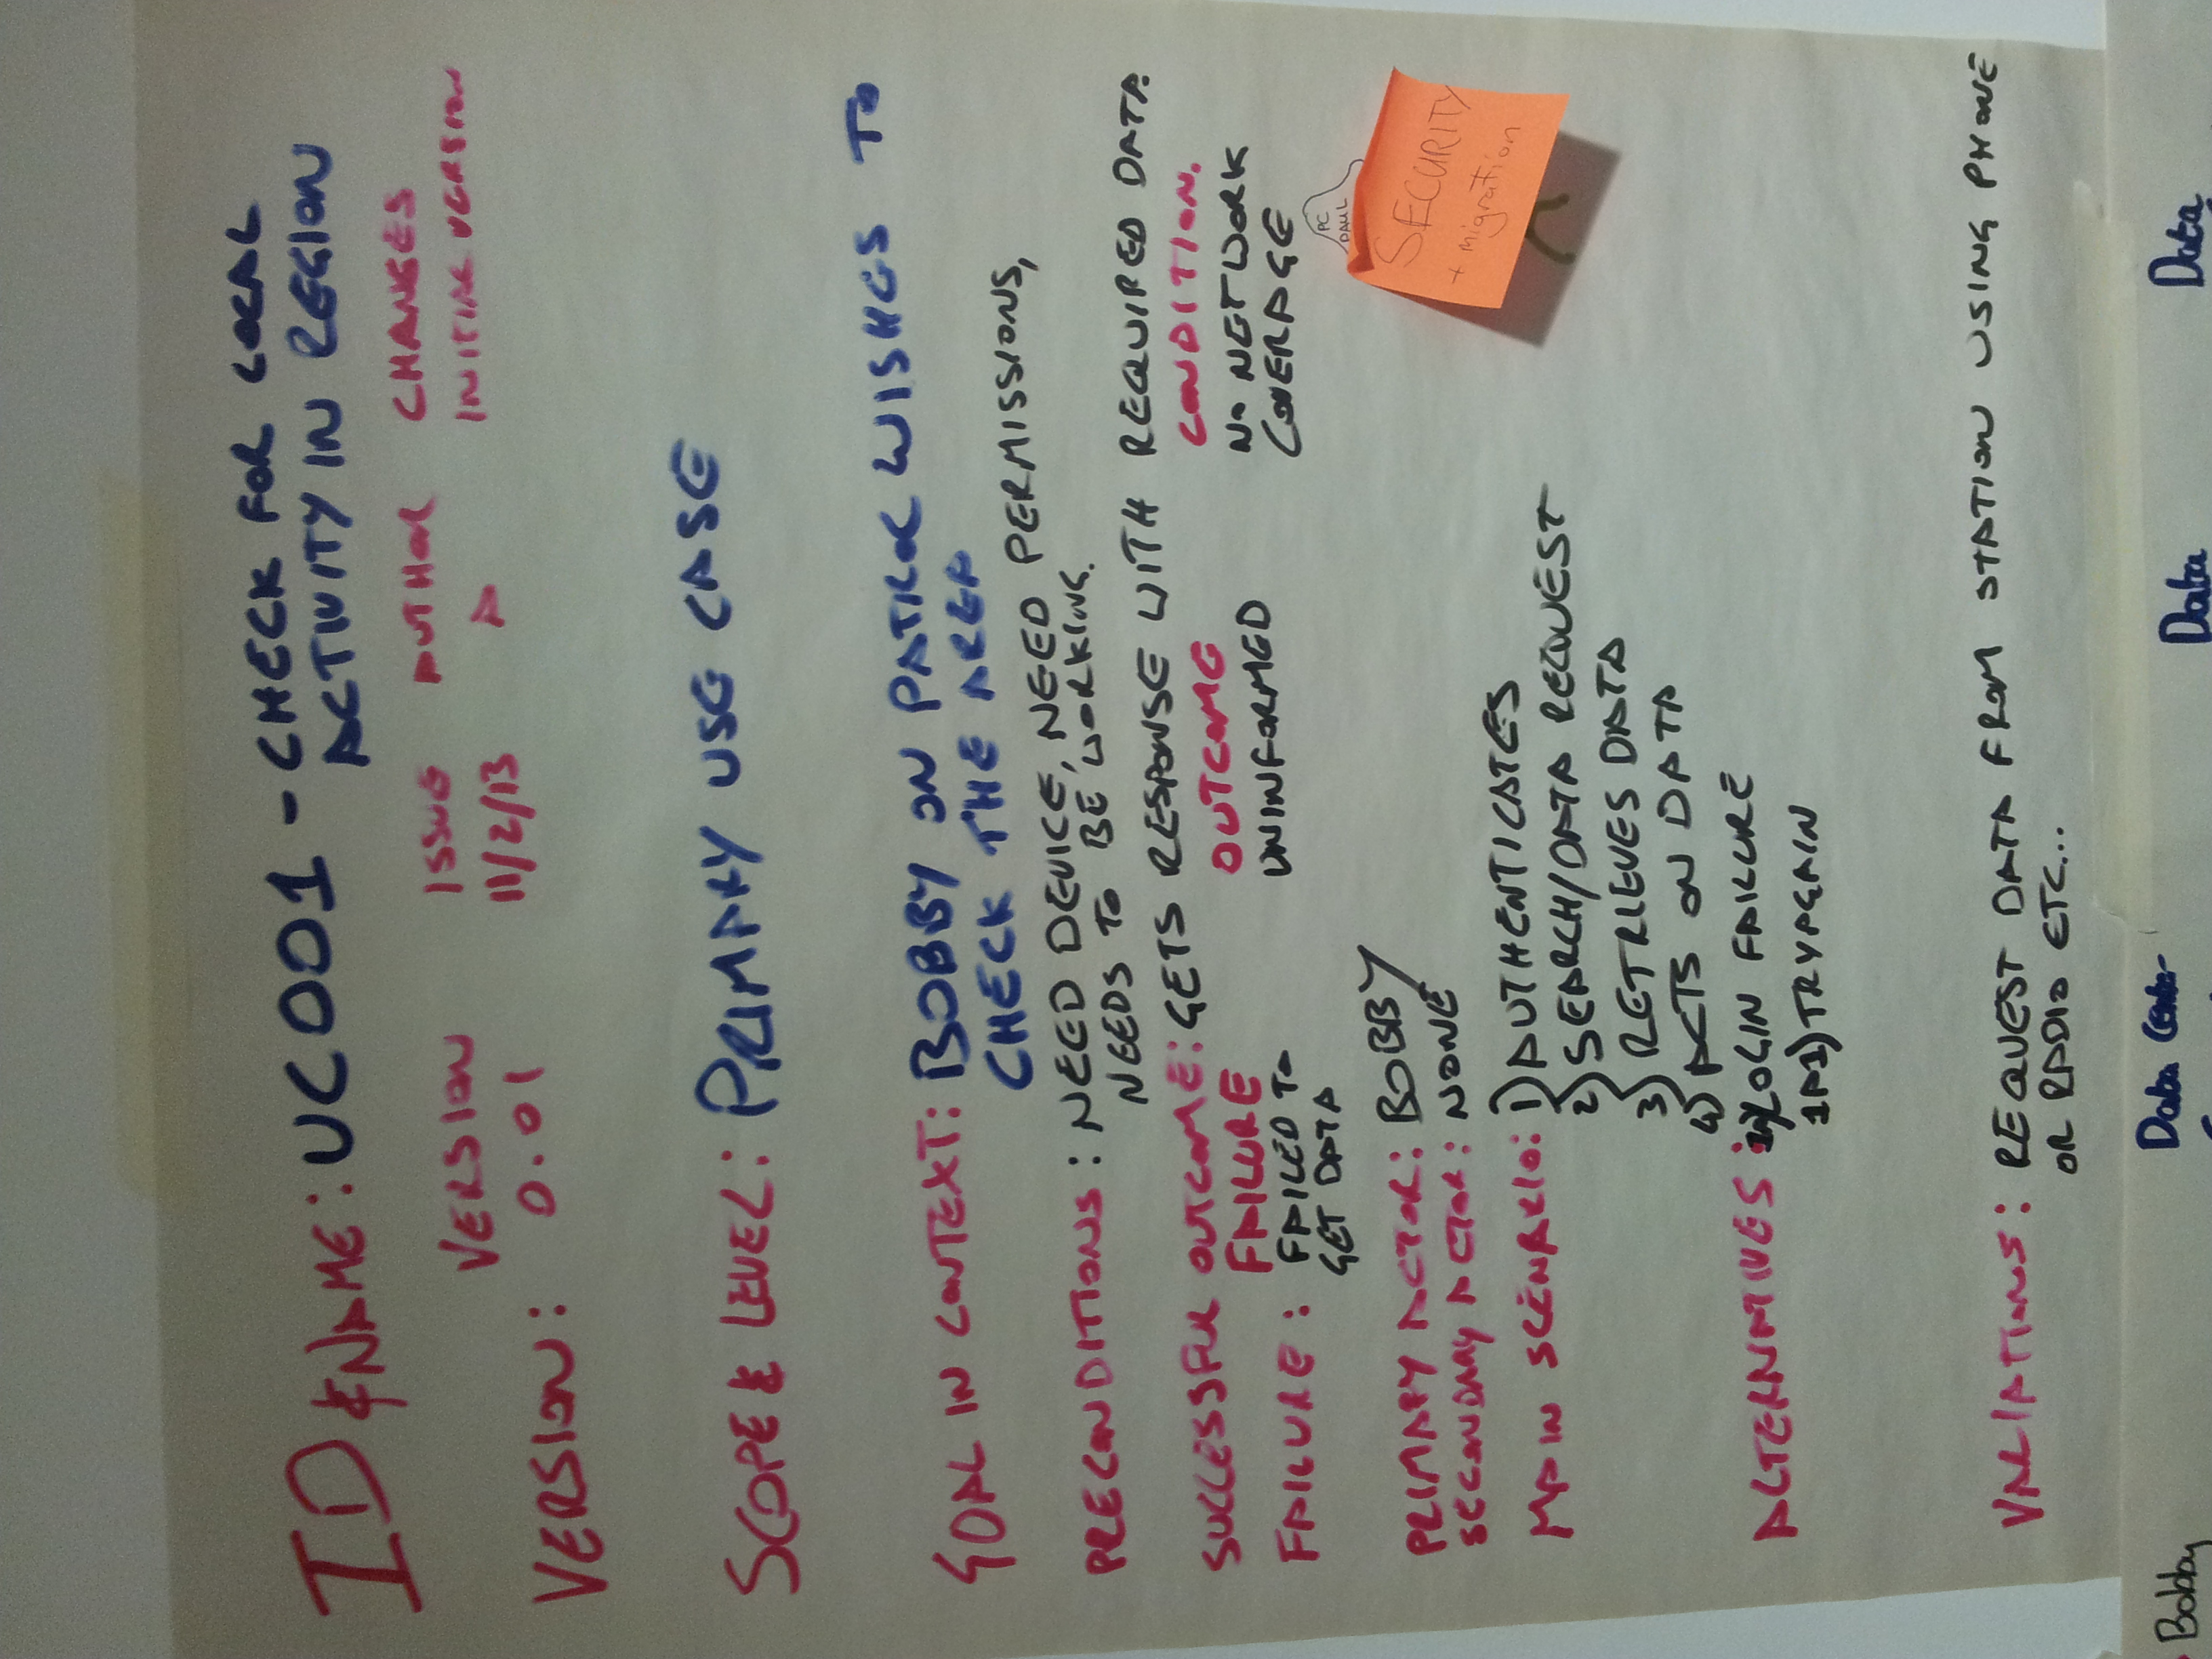
\includegraphics[width=\linewidth, angle=-90]{use-case}
\parbox{0.90\linewidth}{\caption{The use case diagram that I presented}}
\end{center}
\end{wrapfigure}

There were a number of items that I presented during the course of the two sessions, including use case diagrams and sequence diagrams. I found this particularlly challenging as I don't deem presenting to be one of my strongest suits found but found that each subsequent presentation was delivered to a higher standard each time. Another challening aspect was being able to answer the questions by IBM's experts in an accurate and succinct manner, our team adpoted the approach where the person presenting on a subject should also be the first person to answer any questions pertainent to that subject.

\section{The three C's - Context, Communication and Common Sense}
Of these "three C's", by far the most important to me personally is the communication part. As the group was largely reponsible for its own work during the majority of the day, good communication skills were very important. Furthermore, each member of the team was expected to conduct themselves in a professional manner, whilst still maintaining a friendly and approachable demeanour, a feat that I feel each member of the team conformed to in an exemplary fashion. A good example of this was our discussions relating to the architecture overview diagram. Without getting into specifics, there were many varying opinions on how best to go about creating our diagram. One can imagine that in a group of individuals with strong personalities, that such a situation could quickly become volatile and unsavourary. In fact the opposite occurred, everyone conducted themselves in a manner approapriate for the task and all opinions were analysed and acted upon as necessary.

The common sense factor of the "three C's" played a big part when it came to us deciding how exactly to complete the task. It became apparent that not everything could be depicted and communicated solely via the diagrams we were tasked with creating. It was paramount, therefore, that each member of the team knew that the description of these diagrams was equally important as the diagrams themselves. For this reason it was important to occationally step back from the task (for instance when focussing on the minutia of the diagrams), to remember that any indiscrepencies or confusing visual aids are perhaps better explained in person. The same of course is true for university lectures, where it is commonly agreed that attendence at lectures provides a substantially richer experience than reading the material after the lecture has taken place.

\section{Presentations}

This was be far the most stressful part of the project, however, it was very good that we were given an opportunity to present our work twice, allowing for substantial improvement. It is not immediately apparant as to how our revised presentation was a much needed and improved demonstration in quality. This could be as we were under a lot of pressure during the initial presentation and had to present something quickly, that we were not able to produce a first draft that would be to a standard of our linking, additionally it could be due the feedback that we received regarding the presentation.

\begin{wrapfigure}{l}{0.5\textwidth}
\begin{center}
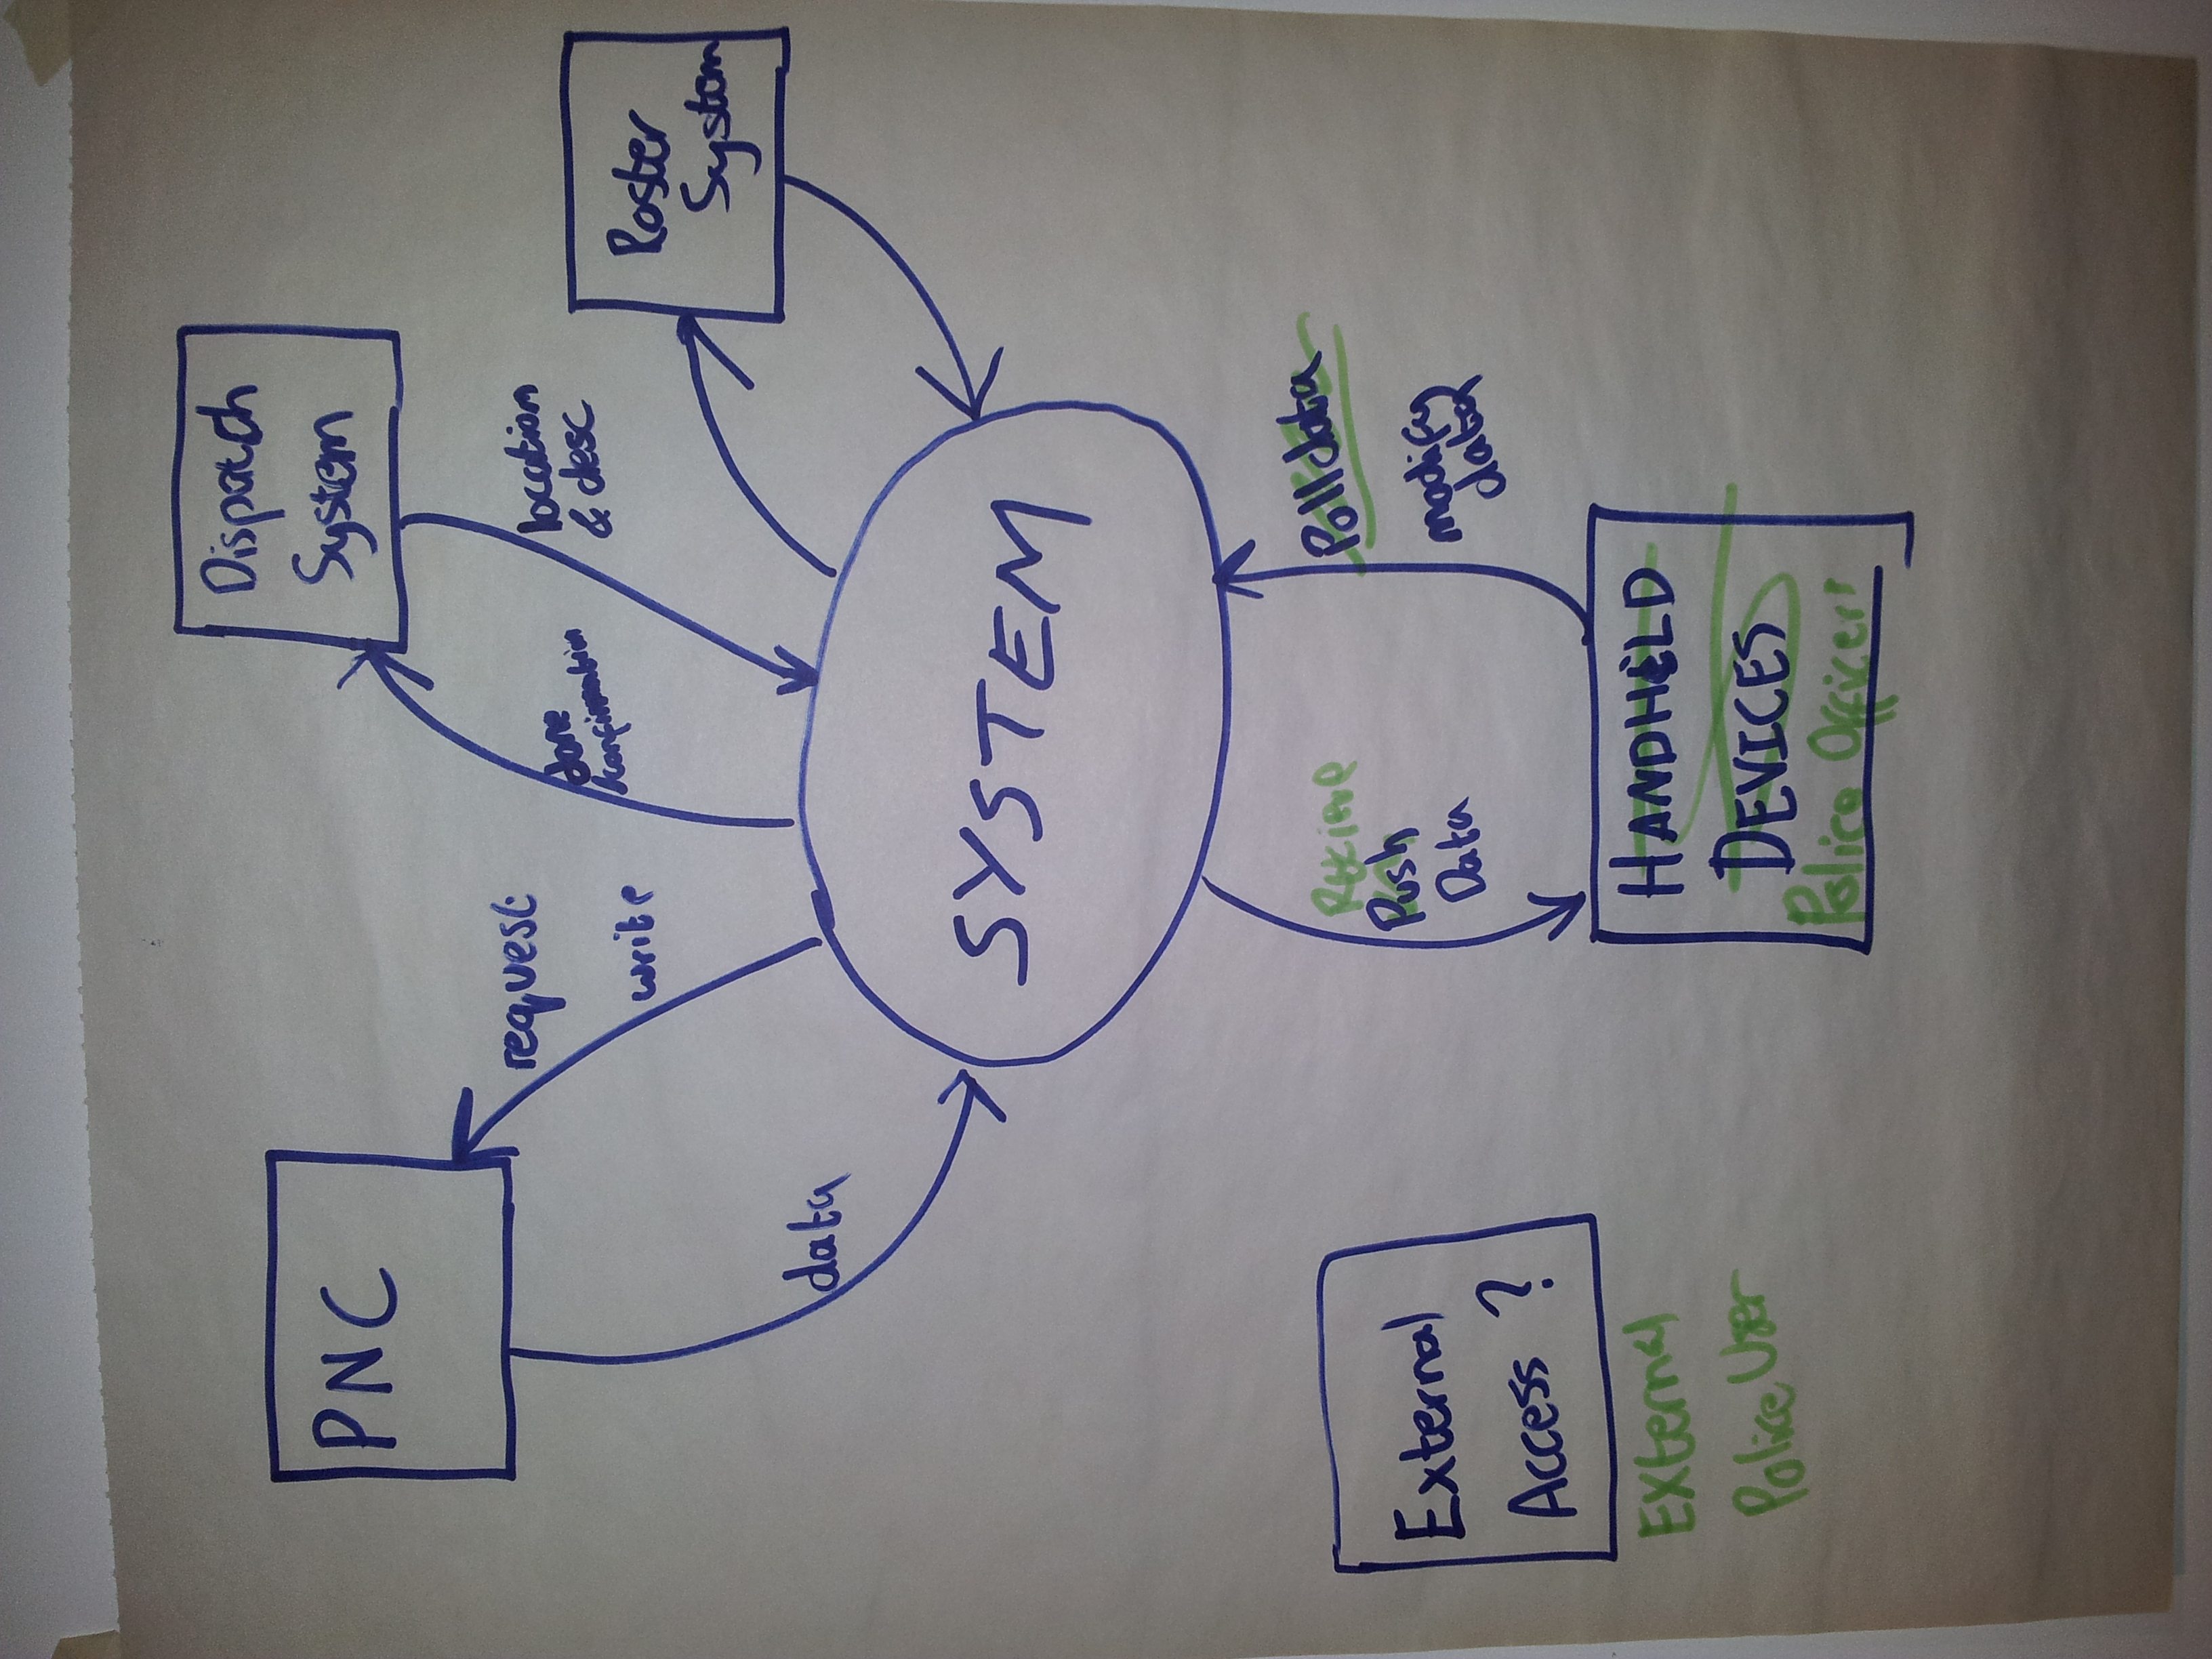
\includegraphics[width=\linewidth, angle=-90]{dia1}
\parbox{0.90\linewidth}{\caption{Our initial system context diagram used in our presentation}}
\end{center}
\end{wrapfigure}

It was remarked afterward that the inclusion of photos of our diagrams was lazy. The reasons we opted to do this were mostly due to the time contraints we had to prepare a draft presentation. Indeed, the week following the presentation we were able to make a much more professional attempt at the diagrams, although, the process was lengthy and almost took the same length of time we had to make our initial presentation (2 hours). Despite the time constraints and limited resources (1 laptop between 6 people), I feel that our initial presentation, whilst not a hallmark of perfection, still provided a reasonable overview of the system we had designed. In addition I felt that we handled the questions quite well, with me answering a majority in both presentations. Interestingly, on that note, our approach to answering questions changed from our initial system (where each person answers questions related to their own slides) to anyone who felt that they could answer the questions well can answer. I was initially skeptical on this as in the past this hasn't worked as it allows people to shy away from questions, with a select few being left to handle their share. However, as the team operated fairly well and there was no one to our knowledge that conformed to such a persona, this changed seemed natural and worked very well during our final presentation.

\section{Conclusion}

In conclusion, the days were very enjoyable and I would have loved to have spent more time getting into much more detail over the systems as I felt that the design aspect was done from a very high level. All members of the IBM team were very friendly and approachable, and as such, were instrumental in our final system design. I always enjoy opportunities that alloy me to exercise my soft skills and team skills, as well as put into practise any knowledge that I have accumilated (in this instance, course content from lectures). 
















\end{document}